% A Provenance-Sealed Anomaly-Score Candidate Catalogue of DESI DR1 Spectra
% Anomaly flagship (Track C2) -- manuscript skeleton
% Houston Golden -- 2026
% Target venue: ApJS (catalogue + method paper with a large public data
% product). Typeset here in revtex4-2, the lab's compile standard
% (/paper-compile-revtex); conversion to AASTeX is a packaging step.
% Every quantitative statement in this file is produced by
% pipelines/p1_highz_tracers/flagship_assembly_2026-09-18/scripts/
% assemble_flagship_evidence.py from the released artifacts; tables under
% tables/ are machine-generated by make_tables.py and must not be edited by
% hand. PLACEHOLDER marks a number that does not exist yet.
% Compile: pdflatex main && pdflatex main && pdflatex main && pdflatex main

\documentclass[aps,prd,twocolumn,superscriptaddress,nofootinbib,longbibliography,floatfix]{revtex4-2}

\usepackage{amsmath,amssymb,amsfonts}
\usepackage{graphicx}
\usepackage{bm}
\PassOptionsToPackage{hyphens}{url}
\usepackage{hyperref}
\usepackage{xcolor}
\usepackage{booktabs}
\usepackage{enumitem}
\usepackage{mathtools}
\usepackage[utf8]{inputenc}

\hypersetup{
  colorlinks=true,
  linkcolor=blue!60!black,
  citecolor=blue!60!black,
  urlcolor=blue!60!black,
  pdfnewwindow=true
}

\newcommand{\paperVersion}{vAF.0.1}
\newcommand{\paperTimestamp}{September 18, 2026}
\newcommand{\repoSHA}{main}
% #1 = repo-relative path (raw, used in the URL); #2 = short display text.
\newcommand{\artifactlink}[2]{\href{https://github.com/Hubify-Projects/bigbounce/blob/\repoSHA/#1}{\texttt{#2}}}
\newcommand{\artifactdirlink}[2]{\href{https://github.com/Hubify-Projects/bigbounce/tree/\repoSHA/#1}{\texttt{#2}}}
\newcommand{\etal}{\textit{et~al.}}
\newcommand{\ZWARN}{\texttt{ZWARN}}
\newcommand{\TARGETID}{\texttt{TARGETID}}
\newcommand{\OBJTYPE}{\texttt{OBJTYPE}}
\newcommand{\TODO}[1]{\textcolor{red}{[\textsc{placeholder}: #1]}}

\begin{document}

\title{A provenance-sealed anomaly-score candidate catalogue of DESI DR1
spectra: selection, validation, and a descriptive taxonomy}

\author{Houston Golden}
\email{houston@hubify.com}
\affiliation{Hubify Research}

\date{\paperTimestamp\ (\paperVersion)}

\begin{abstract}
We publish a machine-flagged candidate catalogue of spectroscopically unusual
objects in Data Release 1 of the Dark Energy Spectroscopic Instrument (DESI),
together with the complete provenance chain needed to reproduce it. An
archived convolutional autoencoder, bound by SHA-256 to a sealed run contract,
assigns a reconstruction-error anomaly score $S$ to every science-target
spectrum in the public \texttt{iron} release; $27{,}547{,}223$ unique
\TARGETID s are scored. We show that a score cut alone does not select
astrophysical objects: above $S=3$, more than $99.5\%$ of raw fibres in every
score bin are sky or non-science fibres, and that fraction \emph{rises} with
score. Applying an explicit science-target provenance gate
($\OBJTYPE = \mathrm{TGT}$, $\texttt{COADD\_FIBERSTATUS} = 0$,
$\TARGETID > 0$) before any score cut, and a pre-declared threshold rule,
yields a released catalogue of $1{,}244$ objects. We validate the catalogue
against a published contract of sixteen machine-checkable requirements, and
report two results that constrain its interpretation: within the
science-target sample the anomaly score is uncorrelated with exposure quality
and source brightness ($|\rho_s| < 0.1$ against median signal-to-noise,
exposure time, \texttt{TSNR2} and $r$-band flux), so the tail is not a
faintness artefact; and the score is driven almost entirely by the blue
spectrograph arm ($\rho_s = +0.53$ against the $b$-camera residual, versus
$-0.04$ and $-0.14$ for $r$ and $z$). Cross-matching against SIMBAD and NED
identifies counterparts for $569$ objects ($45.7\%$); the $675$ unmatched
objects are grouped into a descriptive taxonomy of $25$ clusters and $8$
families, which we show carries no material structure in the model's own
latent space and must therefore be read as a stratification of the candidate
list rather than as physical classes. A known-object recovery benchmark
against five reference classes recovers no class at the pre-declared bar. We
name $32$ follow-up targets in five rules-based tiers --- including four
anomaly-selected DESI-pipeline $z>4$ quasar candidates, two of them at
$z>6$, with no catalogued counterpart --- and list the open tests, led by the
absent selection function, that any population-level use of this catalogue
must clear first.
\end{abstract}

\maketitle

\section{Introduction}
\label{sec:intro}

Wide-field spectroscopic surveys produce far more spectra than can be
inspected. Unsupervised outlier detection is the standard response
\cite{BaronPoznanski2017}, and it works: a model trained to reconstruct
typical spectra flags the ones it cannot. What such a search usually does not
publish is the part that decides whether its output means anything --- the
exact model, the exact code, the exact parent catalogue, the selection rule,
and the reason the rule was chosen.

This paper publishes that part alongside the catalogue. Our primary
deliverable is a scored candidate catalogue of DESI DR1 spectra
\emph{together with} a sealed provenance chain: the SHA-256 of the parent
zcatalog, of the archived model, of the inference code, and of every
intermediate product, bound under one run contract, with a re-runnable gate
for the selection rule and a published validation contract of requirements a
third party can check against the released files.

\TODO{one paragraph placing this among prior DESI/SDSS anomaly-detection
catalogues, cited as prior work; see the release document's neutral
prior-work sentence}

Section~\ref{sec:data} describes the data and the provenance chain,
Sec.~\ref{sec:method} the model and the selection rule,
Sec.~\ref{sec:validation} the validation contract and what it establishes,
Sec.~\ref{sec:catalogue} the catalogue, Sec.~\ref{sec:taxonomy} the
descriptive taxonomy, Sec.~\ref{sec:followup} the named follow-up set and the
open tests, and Sec.~\ref{sec:limits} what this catalogue is not.

\section{Data}
\label{sec:data}

\subsection{DESI DR1}
We use Data Release 1 of DESI \cite{DESIDR1,DESIInstrument}: the public
\texttt{iron} spectroscopic reduction, its redshift catalogue
\texttt{zall-pix-iron.fits} (SHA-256 \texttt{2d95ad99\ldots}), and the
per-(survey, program, healpix) coadd spectra, streamed and scored in place
rather than bulk-downloaded. Redshifts and spectral classifications are the
pipeline's own \cite{DESIPipeline}.

\subsection{Provenance chain}
Every stage binds the exact SHA-256 of its input and output under a single
sealed run contract (generation \texttt{clean-rerun-6699d09ff886}):

\begin{itemize}[leftmargin=1.2em,itemsep=2pt]
  \item parent zcatalog \texttt{2d95ad99\ldots};
  \item $36{,}634$-group locator inventory, receipt-verified group by group;
  \item archived model \texttt{f5266ba4\ldots} and inference code
        \texttt{3e7efb24\ldots};
  \item enrichment, cross-match, and taxonomy manifests, each naming its
        input hash and its output hash.
\end{itemize}

All eight links of that chain are verified in the validation contract
(check V3, Table~\ref{tab:contract}), and all nine released artifacts re-hash
to the values in the landing receipt (check V2).

\section{Method}
\label{sec:method}

\subsection{Anomaly score}
Spectra are scored by an archived autoencoder (a $496 \to 128$ reconstruction
network) frozen for this run; the score is the model's reconstruction-error
statistic, so a high score means a spectrum unlike the shapes the model
learned to reproduce. The scoring pass covered $28{,}425{,}963$ raw rows,
deduplicated by last occurrence to $27{,}547{,}223$ unique \TARGETID s. The
enrichment stage's independent MSE reproduction check passed for all $1{,}244$
released rows with zero offenders (check V3b).

\subsection{Science-target selection}
A row enters the candidate pool only if
$\OBJTYPE = \mathrm{TGT}$ \emph{and} $\texttt{COADD\_FIBERSTATUS} = 0$
\emph{and} $\TARGETID > 0$, the last asserted rather than merely filtered.
This gate is applied \emph{before} any score cut and is enforced by a
committed, re-runnable checker,
\artifactlink{pipelines/p1_highz_tracers/clean_rerun/gates/check_sample_provenance.py}{check\_sample\_provenance.py}
(full path in the reproducibility manifest).

The gate is not a formality. Figure~\ref{fig:skyfraction} shows the fraction
of raw fibres that are sky or non-science as a function of score: it exceeds
$99.5\%$ in every bin above $S=3$ and \emph{increases} with score, from
$99.53\%$ in $[3,4)$ to $99.97\%$ in $[8,10)$. A naive top-score selection
from this scan returns instrument artefacts. Table~\ref{tab:ladder} gives the
raw and science-target counts on the threshold ladder.

\subsection{Threshold rule}
The release threshold follows a rule fixed before the science-only counts were
inspected: from the grid $\{3,4,5,6,8,10\}$, take the largest threshold whose
science-only count is $\ge 300$; if that count exceeds $1{,}500$, step to the
next grid point unless doing so drops the count below $300$. The rule selects
$S>3$ with $n=1{,}244$, reproduced independently in check V4.

\begin{table}[t]
\caption{Threshold ladder: all fibres versus science targets.}
\label{tab:ladder}
\begin{ruledtabular}
\begin{tabular}{r r r r}
$S>$ & All fibres & Science targets & Science fraction \\
\hline
3 & 320{,}418 & 1{,}244 & 0.39\% \\
4 & 86{,}053 & 152 & 0.18\% \\
5 & 52{,}188 & 44 & 0.08\% \\
6 & 27{,}180 & 20 & 0.07\% \\
8 & 3{,}810 & 2 & 0.05\% \\
10 & 337 & 1 & 0.30\% \\
\end{tabular}
\end{ruledtabular}

\end{table}

\begin{figure}[t]
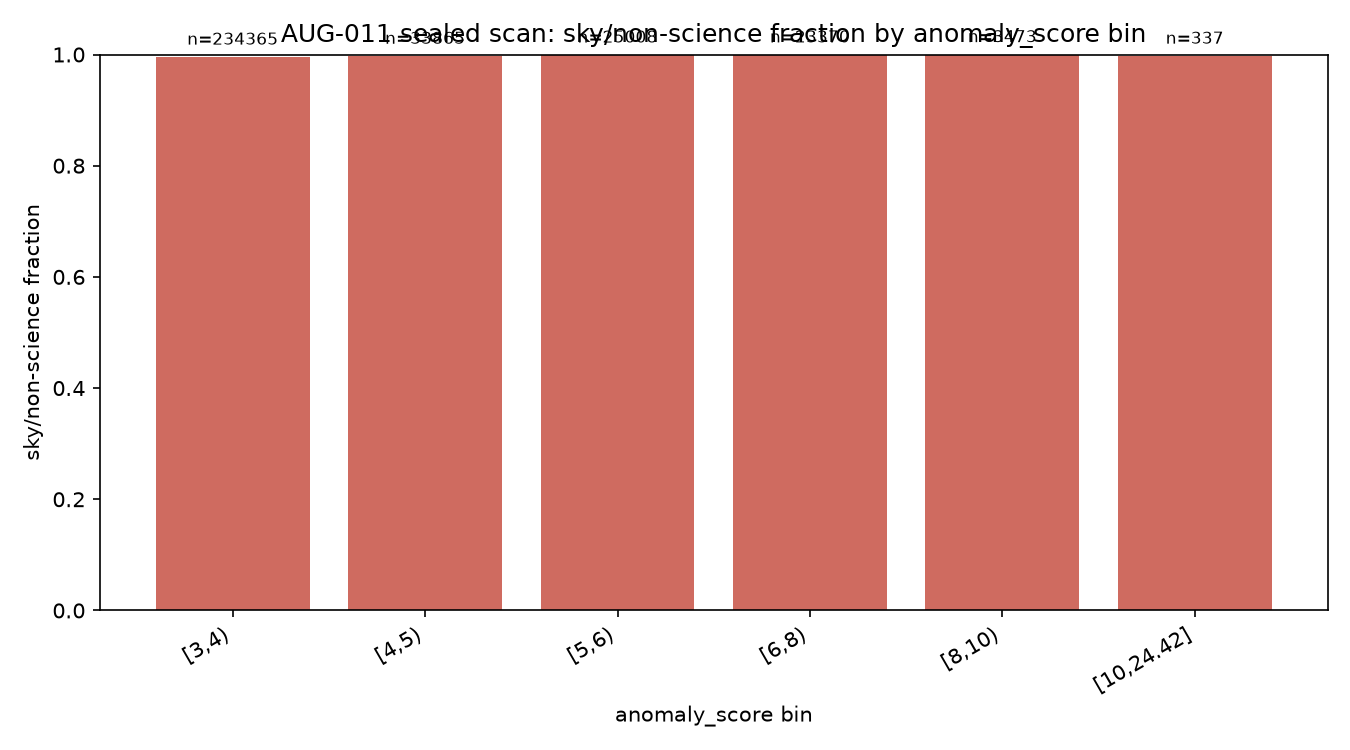
\includegraphics[width=\columnwidth]{figures/sky_fraction_by_score.png}
\caption{Sky-or-non-science fibre fraction as a function of anomaly score,
before the provenance gate. The fraction exceeds $99.5\%$ in every bin above
$S=3$ and rises with score.}
\label{fig:skyfraction}
\end{figure}

\section{Validation}
\label{sec:validation}

\subsection{The validation contract}
Table~\ref{tab:contract} lists the requirements this release is held to. Each
is machine-checkable against the published files; the checker and its raw
output are released with the catalogue. Requirements cover provenance and
hash binding (V1--V3b), the selection rule (V4, V7, V9), internal consistency
of the released tables (V5, V6, V8), and three tests of what the score
measures (V10--V12).

\begin{table*}[t]
\caption{Validation contract. Outcomes are re-run against the released
artifacts; \textsc{reported} marks a quantity the release must state rather
than a threshold it must clear.}
\label{tab:contract}
\begin{ruledtabular}
\begin{tabular}{l p{0.52\textwidth} l}
ID & Requirement & Outcome \\
\hline
V1 & gates/check\_sample\_provenance.py exits 0 on the released sample tables (TARGETID $>$ 0; OBJTYPE/FIBERSTATUS where carried) & \textsc{pass} \\
V2 & every released artifact's SHA-256 equals the value in the landing receipt (PHASE3\_V2\_LANDING\_2026-09-03.md) & \textsc{pass} \\
V3 & the manifest chain closes end to end: sample $\to$ enrichment $\to$ cross-match $\to$ taxonomy, each stage binding the exact SHA-256 of its input and output, under one run contract, with the model / inference-code / zcatalog hashes recorded & \textsc{pass} \\
V3b & the enrichment stage's own MSE reproduction cross-check passed for every released row & \textsc{pass} \\
V4 & replaying the pre-declared threshold rule (largest grid point with science-only count $>$= 300, step up if $>$ 1,500) on the science-target counts selects the released threshold & \textsc{pass} \\
V5 & the cross-match output partitions the sample exactly: matched + unmatched = sample, disjoint, no duplicate TARGETIDs, and the enriched table covers the same TARGETIDs & \textsc{pass} \\
V6 & the taxonomy covers exactly the SIMBAD/NED-unmatched subset; 25 clusters roll up into 8 families; per-family counts sum to the unmatched count and match the per-object labels & \textsc{pass} \\
V7 & every released object exceeds the stated score threshold (S $>$ 3) & \textsc{pass} \\
V8 & the AllWISE table covers every released object and its match count equals the released figure (74) & \textsc{pass} \\
V9 & the released sky-fraction-by-score validation supports the stated claim that every score bin above 3 is $>$ 99.5\% sky-or-nonscience before the provenance gate & \textsc{pass} \\
V10 & within the science-target sample the anomaly score is not a restatement of exposure quality or source brightness ($|$Spearman rho$|$ $<$ 0.2 against S/N, exposure time, TSNR2 and r-band flux) & \textsc{pass} \\
V11 & the per-band residual decomposition identifies which camera arm drives the score (reported, not gated) & \textsc{reported} \\
V12 & the released taxonomy's family partition is tested for structure in the 128-dimensional latent space it was NOT built from (silhouette vs a label-permutation null, 50 draws) & \textsc{structured-but-weak} \\
DEFECT-1 & the enriched table's zcatalog columns (z, zwarn, spectype, subtype) are populated & \textsc{fail} \\
DEFECT-2 & every derived residual-diagnostic column in the enriched table carries values & \textsc{fail} \\
DEFECT-3 & the fraction of released objects carrying a DESI-reliable redshift (ZWARN == 0) is stated with the catalogue & \textsc{reported} \\
\end{tabular}
\end{ruledtabular}

\end{table*}

\subsection{The score is not an exposure-quality proxy}
Within the science-target sample the anomaly score is essentially
uncorrelated with every available measure of how well a spectrum was
measured: Spearman $\rho_s = +0.058$ against median coadd signal-to-noise,
$-0.076$ against coadd exposure time, $-0.093$ and $-0.096$ against
$\texttt{TSNR2}_{\rm LRG}$ and $\texttt{TSNR2}_{\rm QSO}$, and $-0.016$
against $r$-band flux (Fig.~\ref{fig:quality}). At $n=1{,}244$ several of
these are formally significant and all are negligible in size; the two
significant ones are negative, i.e.\ longer exposures score marginally
\emph{lower}. The claim this supports is narrow and negative: the $S>3$ tail
is not explained by faintness or short exposure. It is not evidence that the
tail is astrophysically interesting.

\begin{figure}[t]
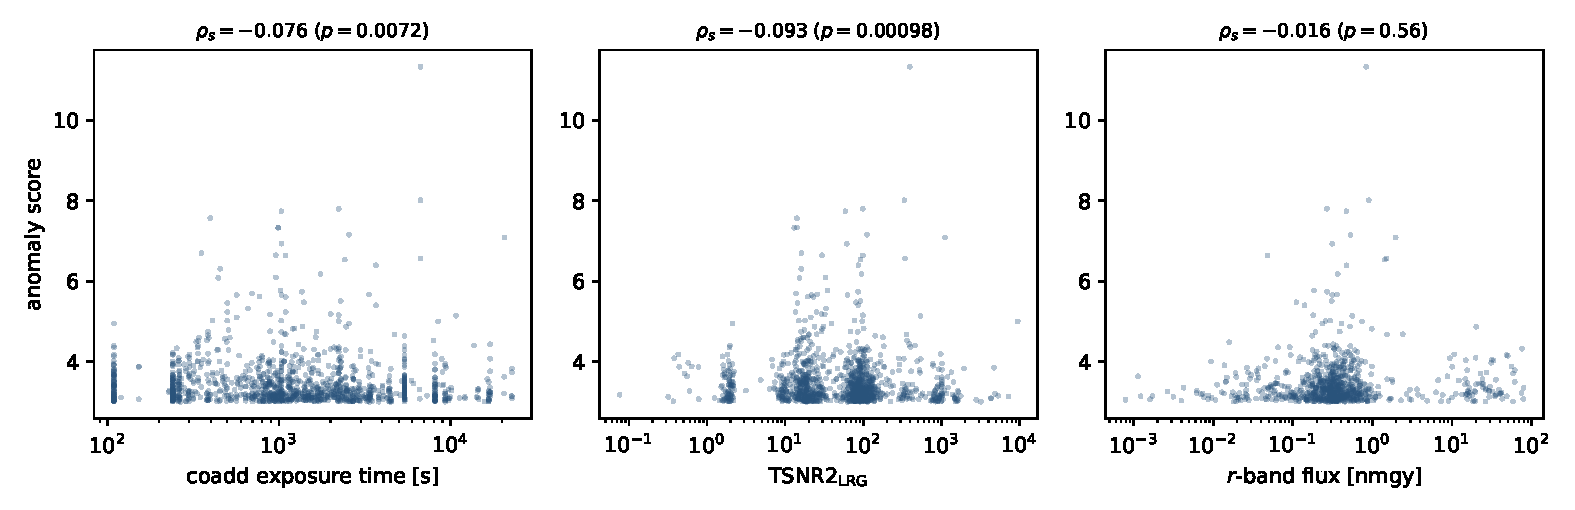
\includegraphics[width=\columnwidth]{figures/fig_score_vs_quality.pdf}
\caption{Anomaly score against exposure time, $\texttt{TSNR2}_{\rm LRG}$, and
$r$-band flux for the $1{,}244$ released objects, with Spearman
coefficients.}
\label{fig:quality}
\end{figure}

\subsection{The score is driven by the blue arm}
Decomposing the reconstruction residual by spectrograph camera gives
$\rho_s(S, r_B) = +0.527$ ($p \sim 10^{-89}$) against $-0.037$ for $r_R$ and
$-0.142$ for $r_Z$. Whatever the model responds to lives in the $b$ camera.
Whether that reflects blue-end sky-subtraction and calibration residuals or
genuine spectral behaviour is the single most consequential open question
about this catalogue, and it is testable on public data
(Sec.~\ref{sec:followup}).

\subsection{Known-object recovery}
Five reference classes with usable positions were cross-matched against the
released sample at $1.5''$ (Table~\ref{tab:recovery}). One broad-absorption-line
quasar matches, at $4.2\times$ the base rate; no other class matches at all.
Against the pre-declared bar --- at least one class at $>10\times$ enrichment
with $\ge 5$ matches --- \emph{no reference class is recovered}. This is the
result that makes the present work a data release with a validated selection
rather than a discovery paper, and we state it as such.

\begin{table*}[t]
\caption{Known-object recovery benchmark, $1.5''$ positional match.}
\label{tab:recovery}
\begin{ruledtabular}
\begin{tabular}{l r r r}
Reference class & $N_{\rm ref}$ in footprint & $N_{\rm match}$ & Enrichment \\
\hline
Broad absorption line (BAL) quasars & 5{,}285 & 1 & 4.2$\times$ \\
Roma-BZCAT blazars (5th ed.) & 2{,}060 & 0 & 0.0$\times$ \\
Cataclysmic variables / WD binaries & 580 & 0 & 0.0$\times$ \\
Lyman-$\alpha$ emitters & 84 & 0 & 0.0$\times$ \\
Superluminous-SN host galaxies & 27 & 0 & 0.0$\times$ \\
\end{tabular}
\end{ruledtabular}

\end{table*}

\section{The catalogue}
\label{sec:catalogue}

The released catalogue contains $1{,}244$ objects, each carrying \TARGETID,
sky position, DESI survey and programme, pipeline redshift and
classification, Legacy Survey photometry, per-band reconstruction residuals,
the $128$ latent activations, and the anomaly score, which ranges from
$3.000$ to $11.332$.

Of the $1{,}244$, $502$ ($40.4\%$) carry a reliable pipeline redshift
($\ZWARN = 0$); the remaining $742$ carry $\ZWARN = 4$
(\texttt{SMALL\_DELTA\_CHI2}) and their redshifts must not be used as
measurements. Every redshift-dependent statement in this paper is restricted
to the $\ZWARN = 0$ subset. Pipeline classifications are $1{,}153$
\texttt{GALAXY}, $86$ \texttt{QSO} and $5$ \texttt{STAR}. AllWISE counterparts
exist for $74$ objects, with median $W1-W2 = 0.51$.

SIMBAD \cite{SIMBAD} and NED cross-matching at $3''$ identifies counterparts
for $569$ objects ($45.7\%$; $562$ via NED, $38$ via SIMBAD, some via both),
leaving $675$ ($54.3\%$) unmatched. Unmatched does not mean new: it includes
objects outside other surveys' footprints or below their detection limits.
Notably, the three highest-scoring objects in the whole sample
($S = 11.33$, $8.01$, $7.80$) are all \emph{matched}, i.e.\ already
catalogued.

\section{Descriptive taxonomy}
\label{sec:taxonomy}

The $675$ unmatched objects are grouped by PCA $\to$ UMAP \cite{UMAP} $\to$
HDBSCAN \cite{HDBSCAN} on $(S, \alpha, \delta)$ into $25$ clusters, rolled up
by descriptor identity into $8$ families (Table~\ref{tab:families},
Fig.~\ref{fig:families}). Family sizes sum to $675$ exactly.

Because the clustering features are the score and the sky position, the
families are in practice a score-tier $\times$ survey/programme
stratification: $70.4\%$ of objects lie in their family's dominant
survey/programme cell, and no family is a compact sky region (the most
concentrated still spans $52^\circ$ in right ascension). We therefore tested
the partition in the space the model actually encodes spectra into: its
silhouette over the $128$ latent dimensions is $-0.016$ against a $50$-draw
label-permutation null of $-0.024 \pm 0.004$ (check V12). The partition is
distinguishable from a random relabelling, but its absolute silhouette is
negative --- the families are \emph{not} separated clusters in latent space.
They are reported as descriptive strata, carry descriptor labels only, and no
family is given a physical class name.

Two families stand out for follow-up purposes. Family~3 ($61$ objects, single
cluster) is the extreme-score family, with median $S = 4.38$, the largest
median blue residual of any family, and the highest-scoring unmatched object
in the catalogue ($S = 7.15$). Family~6 ($36$ objects) has the highest
reliable-redshift fraction ($75\%$) at an elevated score and no object above
$z = 2$: well-measured, low-redshift, high-score, and therefore the family in
which an instrumental or template explanation is most directly testable.

\begin{table*}[t]
\caption{Per-family evidence over the $675$ SIMBAD/NED-unmatched objects.
$N_{\rm cl}$ is the number of source clusters, $r_B$ the median $b$-camera
residual, $N_{Z0}$ the number with $\ZWARN = 0$, $\tilde z_{Z0}$ their median
redshift, and $N_W$ the number with an AllWISE counterpart.}
\label{tab:families}
\begin{ruledtabular}
\begin{tabular}{r l r r l l r r r r r r}
Family & Tier & $N$ & $N_{\rm cl}$ & Survey/prog. & Score med. (5--95\%) & $r_B$ & $N_{Z0}$ & $\tilde z_{Z0}$ & $N_{z>2}$ & $N_{\rm QSO}$ & $N_{W}$ \\
\hline
0 & low & 302 & 12 & main/dark & 3.14 (3.02--3.38) & 2.42 & 144 & 1.15 & 13 & 18 & 0 \\
1 & elevated & 87 & 4 & main/dark & 3.35 (3.12--3.78) & 2.53 & 47 & 1.20 & 8 & 10 & 1 \\
2 & elevated & 71 & 2 & sv3/bright & 3.53 (3.35--4.06) & 2.60 & 18 & 1.36 & 2 & 4 & 2 \\
3 & extreme & 61 & 1 & sv3/bright & 4.38 (3.55--6.31) & 2.98 & 19 & 1.19 & 1 & 2 & 1 \\
4 & low & 44 & 2 & sv3/bright & 3.10 (3.01--3.23) & 2.42 & 12 & 1.36 & 3 & 3 & 1 \\
5 & low & 38 & 2 & sv1/other & 3.12 (3.01--3.28) & 2.20 & 15 & 1.01 & 2 & 4 & 1 \\
6 & high & 36 & 1 & main/dark & 3.62 (3.44--4.31) & 2.81 & 27 & 1.09 & 0 & 1 & 0 \\
7 & high & 36 & 1 & sv3/bright & 3.66 (3.37--4.01) & 2.66 & 7 & 0.93 & 0 & 0 & 0 \\
\end{tabular}
\end{ruledtabular}

\end{table*}

\begin{figure}[t]
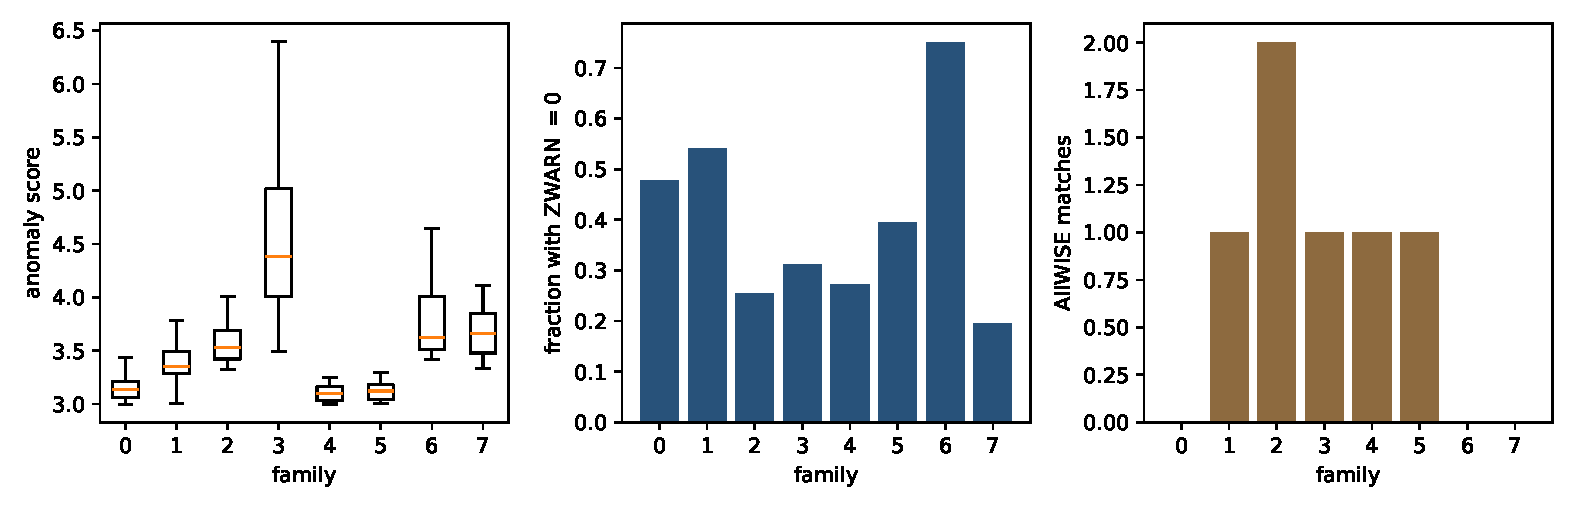
\includegraphics[width=\columnwidth]{figures/fig_family_evidence.pdf}
\caption{Per-family anomaly-score distribution, reliable-redshift fraction,
and AllWISE match count.}
\label{fig:families}
\end{figure}

\section{Follow-up set and open tests}
\label{sec:followup}

\subsection{Named targets}
Table~\ref{tab:followup} names $32$ objects in five rules-based tiers, all
drawn from the unmatched subset. The rules are literature-motivated and
replayable from the released files.

\begin{itemize}[leftmargin=1.2em,itemsep=2pt]
  \item \textbf{FT-A} (4 targets) --- $\ZWARN = 0$ and $z \ge 4$: four
        anomaly-selected DESI-pipeline $z>4$ quasar candidates with no
        catalogued counterpart, two of them at $z > 6$. These are pipeline
        redshifts, not confirmations. The cheapest discriminating test costs
        nothing: a $z>6$ quasar must be a $g$-dropout, so Legacy Survey DR10
        $grz$ photometry \cite{LegacySurveys} at these coordinates refutes or
        supports each one on public data alone, before any spectroscopy.
  \item \textbf{FT-B} (1 target) --- AllWISE $W1-W2 \ge 0.8$, the standard
        mid-infrared AGN criterion \cite{Stern2012,WISE}. Next tests are
        public archives: NEOWISE-R light curve \cite{NEOWISE}, ZTF optical
        light curve \cite{ZTF}, archival X-ray coverage.
  \item \textbf{FT-C} (5 targets) --- $\ZWARN = 0$, $\Delta\chi^2 > 25$ and
        $S$ in the top $5\%$: spectra that are simultaneously well measured
        and hardest to reconstruct, where a genuine spectral anomaly is most
        likely. Three of the five are in family~3.
  \item \textbf{FT-D} (0 targets) --- unmatched point sources with a Gaia DR3
        counterpart \cite{GaiaDR3}. The rule returns nothing: the unmatched
        population is fainter than Gaia's limit throughout. We retain the
        rule so that a deeper generation can re-run it.
  \item \textbf{FT-E} (25 targets) --- the highest-score member of each
        cluster, so that a follow-up programme tests the taxonomy rather than
        one corner of it.
\end{itemize}

\begin{table*}[t]
\caption{Named follow-up targets. $S$ is the anomaly score. Redshifts are
DESI pipeline values and are printed only where $\ZWARN = 0$; a dash marks an
object whose fit carries $\ZWARN = 4$ (\texttt{SMALL\_DELTA\_CHI2}), for which
the pipeline redshift is not a measurement. The FT-E tier spans the taxonomy
by construction and therefore includes such objects.}
\label{tab:followup}
\begin{ruledtabular}
\begin{tabular}{l r r r r r r l}
Tier & TARGETID & R.A. & Dec. & $S$ & $z$ & ZWARN & SPECTYPE \\
\hline
FT-A & 39627903570285763 & 247.89529 & 4.66991 & 3.496 & 6.0878 & 0 & QSO \\
FT-A & 39627607293039577 & 201.10137 & -7.55334 & 3.232 & 6.0638 & 0 & QSO \\
FT-A & 39628216868014338 & 239.92839 & 18.01577 & 3.061 & 5.1938 & 0 & QSO \\
FT-A & 39627849358909321 & 252.47160 & 2.60073 & 3.033 & 4.3338 & 0 & QSO \\
FT-B & 103610381762578 & 223.91434 & 50.21732 & 3.105 & -- & 4 & GALAXY \\
FT-C & 39627812453222421 & 212.59529 & 0.92095 & 7.151 & 1.0798 & 0 & GALAXY \\
FT-C & 39627812461610773 & 213.07783 & 0.96584 & 6.394 & 1.1868 & 0 & GALAXY \\
FT-C & 39627877817258319 & 149.92219 & 3.77396 & 6.180 & 1.1989 & 0 & GALAXY \\
FT-C & 39633001079899014 & 217.98717 & 36.00150 & 4.747 & 1.3533 & 0 & GALAXY \\
FT-C & 39633407088529181 & 97.49930 & 61.65664 & 4.642 & 1.3098 & 0 & GALAXY \\
FT-E & 39627812453222421 & 212.59529 & 0.92095 & 7.151 & 1.0798 & 0 & GALAXY \\
FT-E & 39633407088529181 & 97.49930 & 61.65664 & 4.642 & 1.3098 & 0 & GALAXY \\
FT-E & 39636182677589446 & 64.05184 & -16.74091 & 4.321 & 0.0063 & 0 & GALAXY \\
FT-E & 1071051379310604 & 240.34378 & 42.49037 & 4.289 & -- & 4 & GALAXY \\
FT-E & 39627748041295714 & 333.31949 & -1.73961 & 4.252 & 1.4203 & 0 & GALAXY \\
FT-E & 39628291237221824 & 260.29164 & 21.13162 & 4.108 & -- & 4 & GALAXY \\
FT-E & 39633396858619848 & 275.81585 & 60.77425 & 3.877 & -- & 4 & QSO \\
FT-E & 1070259272417281 & 210.20609 & 6.12193 & 3.762 & -- & 4 & GALAXY \\
FT-E & 1070185960177669 & 150.13551 & 2.91550 & 3.498 & -- & 4 & GALAXY \\
FT-E & 39627903570285763 & 247.89529 & 4.66991 & 3.496 & 6.0878 & 0 & QSO \\
FT-E & 67803973419009 & 130.11975 & 18.65811 & 3.491 & -- & 4 & GALAXY \\
FT-E & 39633418778053415 & 143.59822 & 62.82238 & 3.416 & 1.3659 & 0 & GALAXY \\
FT-E & 39628330143583760 & 240.61454 & 22.94852 & 3.400 & 3.1050 & 0 & QSO \\
FT-E & 39633432057219468 & 96.54153 & 63.88652 & 3.387 & 0.9304 & 0 & GALAXY \\
FT-E & 39633495382820413 & 102.70638 & 70.64374 & 3.334 & -- & 4 & GALAXY \\
FT-E & 39633466035275117 & 293.95821 & 67.33832 & 3.330 & 1.4545 & 0 & GALAXY \\
FT-E & 39627817989705740 & 182.69435 & 1.34328 & 3.325 & 1.2954 & 0 & GALAXY \\
FT-E & 2394988512018434 & 203.98955 & 49.98956 & 3.295 & -- & 4 & GALAXY \\
FT-E & 39633062929108448 & 182.23513 & 39.17878 & 3.279 & 0.2303 & 0 & GALAXY \\
FT-E & 39632946235181990 & 213.68195 & 33.19121 & 3.278 & -- & 4 & GALAXY \\
FT-E & 1070090426515458 & 215.89907 & -1.05994 & 3.247 & -- & 4 & GALAXY \\
FT-E & 39627778101872111 & 325.03381 & -0.42236 & 3.220 & 1.0189 & 0 & GALAXY \\
FT-E & 2394624320602116 & 188.48854 & 30.29515 & 3.216 & -- & 4 & GALAXY \\
FT-E & 39633184245159076 & 270.34970 & 45.93852 & 3.194 & 1.4010 & 0 & GALAXY \\
FT-E & 39627654445405293 & 147.36232 & -5.59562 & 3.158 & -- & 4 & GALAXY \\
\end{tabular}
\end{ruledtabular}

\end{table*}

\subsection{Open tests}
\begin{description}[leftmargin=0em,itemsep=2pt]
  \item[OT-1 Selection function.] No injection-recovery experiment has been
    run for this model on this substrate. The catalogue therefore has no
    measured completeness or purity, and no population-level inference may be
    drawn from it. This is the gate any rate, abundance, or cosmological use
    must clear first. \TODO{run and report per-class injection recovery with
    the exact model and substrate named}
  \item[OT-2 Latent-space taxonomy.] Re-clustering on the $128$ latent
    dimensions rather than on $(S, \alpha, \delta)$.
  \item[OT-3 Blue-arm diagnosis.] Compare the $b$-camera residual against
    airmass, lunar phase, and blue-end sky-subtraction residuals in the DR1
    exposure tables, to separate calibration from astrophysics.
  \item[OT-4 Wider recovery benchmark.] Six of eleven candidate reference
    classes lacked usable positions and were not tested.
  \item[OT-5 Deeper scan.] A self-supervised model trained on the full
    science-target spectrum population, rather than a $47$k-spectrum
    autoencoder, is the realistic route to a confirmed anomalous class.
\end{description}

\section{Data availability and reproducibility}
\label{sec:repro}

The catalogue, its manifests, the validation checker and its output, the
per-family evidence tables, and the follow-up set are released in the project
repository under
\artifactdirlink{pipelines/p1_highz_tracers/clean_rerun/results_2026-08-07/phase3_v2}{results\_2026-08-07/}\-\artifactdirlink{pipelines/p1_highz_tracers/clean_rerun/results_2026-08-07/phase3_v2}{phase3\_v2}
and
\artifactdirlink{pipelines/p1_highz_tracers/flagship_assembly_2026-09-18}{flagship\_assembly\_}\-\artifactdirlink{pipelines/p1_highz_tracers/flagship_assembly_2026-09-18}{2026-09-18}
(both under \texttt{pipelines/p1\_highz\_tracers/}), with mirrors on Hugging
Face and Backblaze B2 verified by checksum. The reproducibility manifest ---
external data sources and links, scripts, compute venue, cost, and wall-clock
--- is
\artifactlink{pipelines/p1_highz_tracers/anomaly_flagship_draft/REPRODUCIBILITY_MANIFEST.md}{REPRODUCIBILITY\_}\-\artifactlink{pipelines/p1_highz_tracers/anomaly_flagship_draft/REPRODUCIBILITY_MANIFEST.md}{MANIFEST.md}.
\TODO{Zenodo DOI for the public deposit}

Two defects in the released tables are recorded openly and must be repaired
before public deposit: the enriched table's \texttt{z}, \ZWARN,
\texttt{SPECTYPE} and \texttt{SUBTYPE} columns are unpopulated (the
authoritative values are in the sample table and are re-joined for every
number in this paper), and \texttt{residual\_kurtosis} is empty. The public
release must ship the joined table. The released files also do not carry
\OBJTYPE\ and \texttt{COADD\_FIBERSTATUS}, so the provenance gate cannot
re-verify those two conditions from the published file alone; both columns
should be carried in the deposit.

\section{What this catalogue is not}
\label{sec:limits}

\begin{itemize}[leftmargin=1.2em,itemsep=2pt]
  \item It is not a discovery catalogue. No object here is reported as a
    confirmed unusual source; selection-pipeline output alone never promotes
    an object to notable.
  \item It is not a statistically characterised sample. Without OT-1 there is
    no completeness, no purity, and no selection function, so no population
    inference is available.
  \item Its families are not physical classes (Sec.~\ref{sec:taxonomy}).
  \item Its unmatched fraction is not a novelty fraction: it includes objects
    simply outside other surveys' footprints or detection limits.
  \item Its anomaly score is a distance from one model's learned
    reconstruction, not a physically motivated significance.
\end{itemize}

\section{Conclusions}
\label{sec:conclusions}

We publish $1{,}244$ DESI DR1 science-target spectra selected by
reconstruction-error anomaly score, with a sealed provenance chain, a
published validation contract, a descriptive taxonomy of the unmatched
subset, and a named follow-up set. Three results are worth carrying forward
independently of the catalogue: a score cut without a provenance gate selects
sky fibres, not objects, and the contamination worsens with score; within the
science-target sample the score is not a proxy for exposure quality or
brightness; and the score is driven by the blue spectrograph arm, which
localises both the next methodological test and the most plausible
instrumental explanation. The known-object recovery benchmark does not clear
its pre-declared bar, and we report the work as what it is --- reproducible
data infrastructure with a validated selection --- rather than as a discovery.

\begin{acknowledgments}
\TODO{DESI collaboration and facility acknowledgements; SIMBAD/NED/VizieR
service acknowledgements; compute acknowledgement}
\end{acknowledgments}

\begin{thebibliography}{99}

\bibitem{BaronPoznanski2017} D.~Baron and D.~Poznanski,
  ``The weirdest SDSS galaxies: results from an outlier detection algorithm,''
  Mon.\ Not.\ R.\ Astron.\ Soc.\ \textbf{465}, 4530 (2017).

\bibitem{DESIDR1} DESI Collaboration,
  ``Data Release 1 of the Dark Energy Spectroscopic Instrument,''
  arXiv:2503.14745 (2025).

\bibitem{DESIInstrument} DESI Collaboration,
  ``Overview of the Instrumentation for the Dark Energy Spectroscopic
  Instrument,'' Astron.\ J.\ \textbf{164}, 207 (2022).

\bibitem{DESIPipeline} J.~Guy \etal,
  ``The Spectroscopic Data Processing Pipeline for the Dark Energy
  Spectroscopic Instrument,'' Astron.\ J.\ \textbf{165}, 144 (2023).

\bibitem{SIMBAD} M.~Wenger \etal,
  ``The SIMBAD astronomical database,''
  Astron.\ Astrophys.\ Suppl.\ Ser.\ \textbf{143}, 9 (2000).

\bibitem{UMAP} L.~McInnes, J.~Healy, and J.~Melville,
  ``UMAP: Uniform Manifold Approximation and Projection for Dimension
  Reduction,'' arXiv:1802.03426 (2018).

\bibitem{HDBSCAN} R.~J.~G.~B.~Campello, D.~Moulavi, and J.~Sander,
  ``Density-based clustering based on hierarchical density estimates,''
  in \textit{PAKDD 2013}, Lecture Notes in Computer Science \textbf{7819},
  160 (2013).

\bibitem{Stern2012} D.~Stern \etal,
  ``Mid-infrared selection of active galactic nuclei with the
  Wide-field Infrared Survey Explorer. I.,''
  Astrophys.\ J.\ \textbf{753}, 30 (2012).

\bibitem{WISE} E.~L.~Wright \etal,
  ``The Wide-field Infrared Survey Explorer (WISE): mission description and
  initial on-orbit performance,'' Astron.\ J.\ \textbf{140}, 1868 (2010).

\bibitem{NEOWISE} A.~Mainzer \etal,
  ``Initial performance of the NEOWISE reactivation mission,''
  Astrophys.\ J.\ \textbf{792}, 30 (2014).

\bibitem{LegacySurveys} A.~Dey \etal,
  ``Overview of the DESI Legacy Imaging Surveys,''
  Astron.\ J.\ \textbf{157}, 168 (2019).

\bibitem{GaiaDR3} Gaia Collaboration,
  ``Gaia Data Release 3: summary of the content and survey properties,''
  Astron.\ Astrophys.\ \textbf{674}, A1 (2023).

\bibitem{ZTF} E.~C.~Bellm \etal,
  ``The Zwicky Transient Facility: system overview, performance, and first
  results,'' Publ.\ Astron.\ Soc.\ Pac.\ \textbf{131}, 018002 (2019).

\end{thebibliography}

\end{document}
